\section{Évaluation}
\label{sec:evaluation}
  Pour valider notre approche, nous réalisons une première série d'évaluations
  visant à déterminer la configuration optimale de TopicRank. Nous comparons 
  ensuite TopicRank aux travaux précédents et analysons l'impact de chacune de
  nos contributions.

  \subsection{Cadre expérimental}
  \label{subsec:cadre_experimental}
    \subsubsection{Méthodes de référence pour l'extraction de termes-clés}
    \label{subsubsec:systemes_de_reference_pour_l_extraction_de_termes_cles}
      % Comment les baselines sont-elles choisies ?
      Dans nos expérimentations, nous comparons TopicRank avec trois autres
      méthodes non-supervisées d'extraction automatique de termes-clés. Nous
      choisissons TextRank et SingleRank, les deux méthodes qui sont la
      fondation des méthodes à base de graphe, et la pondération TF-IDF. Cette
      dernière consiste à donner un score aux termes-clés candidats en faisant
      la somme des poids TF-IDF des mots qui les composent, puis à sélectionner
      ceux ayant le plus haut score.

      % Quelles sont les particularités liées à notre implémentation ?
      Au même titre que pour TopicRank, nous proposons une implémentation des
      méthodes de référence disponible sur la plate-forme de développement
      collaboratif
      GitHub\footnote{\url{https://github.com/adrien-bougouin/KeyBench/tree/ijcnlp_2013}}.
      Dans un souci de comparaison, lorsque les méthodes de référence partagent
      le même comportement que TopicRank, celui-ci est réaliser par le même
      composant.

    \subsubsection{Collections de données}
    \label{subsubsec:donnees_de_test}
      Afin de suivre \newcite{hassan2010conundrums} qui soulignent l'importance
      d'évaluer une méthode avec des collections de données aux configurations
      différentes pour mieux observer et comprendre son comportement, les
      collections de données utilisées dans ce travail diffèrent en termes de
      langue, nature, taille des documents et types d'annotateur (auteurs,
      lecteurs ou les deux).

      \textbf{DUC}~\cite{over2001duc} est une collection en anglais issue des
      données de la campagne d'évaluation DUC-2001. Cette campagne d'évaluation
      concerne les méthodes de résumé automatique, elle ne contient donc
      originellement pas d'annotations en termes-clés. Cependant, les 308
      articles journalistiques de la partie test de DUC-2001 ont été annotés par
      \newcite{wan2008expandrank}. Nous utilisons ces 308 documents pour la
      comparaison de TopicRank avec les méthodes de référence.

      \textbf{SemEval}~\cite{kim2010semeval} est la collection en anglais
      fournie lors de la campagne d'évaluation SemEval-2010 pour la tâche
      d'extraction automatique de termes-clés. Cette collection contient 244
      articles scientifiques (conférences et ateliers) issus de la librairie
      numérique ACM. La collection est répartie en deux sous-ensembles, un
      ensemble de 144 documents d'entraînement et un ensemble de 100 documents
      de test. Lors de nos expériences, nous utilisons les 144 documents
      d'entraînement pour paramétrer TopicRank et SingleRank, et les 100
      documents de l'ensemble de test pour la comparaison de TopicRank avec les
      méthodes de référence. En ce qui concerne les termes-clés associés aux
      documents, ils correspondent à la combinaison de ceux donnés par les
      auteurs et des lecteurs.

      \textbf{WikiNews}\footnote{\url{https://github.com/adrien-bougouin/WikinewsKeyphraseCorpus}}
      est une collection de 100 articles journalistiques en français que nous
      avons extraits du site Web
      WikiNews\footnote{\url{http://fr.wikinews.org}} entre les mois de mai et
      décembre 2012. Pour l'annotation en termes-clés, nous avons demandé à \textcolor{red}{???}
      étudiants de master en TAL d'extraire (librement) les termes-clés de \textcolor{red}{???}
      documents. Chaque document à été annoté par au moins trois étudiants, pour
      un accord inter-annotateurs de \textcolor{red}{???} selon le coefficient
      \textcolor{red}{???}~\cite{doe1942paper}. Nous utilisons les 308 documents de Wikinews pour
      la comparaison de TopicRank avec les méthodes de référence.

      \textbf{DEFT}~\cite{paroubek2012deft} est la collection fournie lors de la
      campagne d'évaluation DEFT-2012 pour la tâche d'extraction automatique de
      termes-clés. Celle-ci contient 234 documents en français issus de quatre
      revues de Sciences Humaines et Sociales. La collection est divisée en deux
      sous-ensembles, un ensemble d'entraînement contenant 141 documents et un
      ensemble de test contenant 93 documents. Lors de nos expériences, nous
      utilisons les 141 documents d'entraînement pour paramétrer TopicRank et
      SingleRank, et les 93 documents de l'ensemble de test pour la comparaison
      de TopicRank avec les méthodes de référence. Seuls les termes-clés des
      auteurs sont disponibles pour cette collection.

      Le tableau~\ref{tab:donnees_de_test} donne les statistiques extraites des
      ensembles de test des quatre collections de données présentées ci-dessus.
      Les données sont divisées en deux langues (anglais et français), avec pour
      chaque langue une collection de documents courts (articles
      journalistiques) et une collection de documents de plus grande taille
      (articles scientifiques). Il est aussi important de noter qu'en fonction
      du type d'annotateurs, le nombre de termes-clés associés varie, de même
      que le nombre de termes-clés n'apparaissant pas dans les documents.
      \begin{table}
        \centering
        \begin{tabular}{@{~}r@{~~}c@{~~}c@{~~}c@{~~}c@{~}}
          \toprule
          \textbf{Statistique} & \textbf{DUC} & \textbf{SemEval} & \textbf{WikiNews} & \textbf{DEFT}\\
          \midrule
          Langue & Anglais & Anglais & Français & Français\\
          Nature & Journalistique & Scientifique & Journalistique & Scientifique\\
          \multirow{3}{*}[.35em]{Annotateurs} & \multirow{3}{*}[.35em]{Lecteurs} & Auteurs & \multirow{3}{*}[.35em]{Lecteurs} & \multirow{3}{*}[.35em]{Auteurs}\\
          \addlinespace[-.7\defaultaddspace]
          & & \& & &\\
          \addlinespace[-.7\defaultaddspace]
          & & Lecteurs & &\\
          Documents & 308 & 100 & 100 & 93\\
          Mos/document & 900,7 & 5177,7 & 308,5 & 6839,4\\
          Termes-clés/document & 8,1 & 14,7 & 9,6 & 5,2\\
          Mots/termes-clés & 2,1 & 2,1 & 1,7 & 1,6\\
          %Termes-clés manquants & 3,5\% & 22,1\% & 7,6\% & 21,1\% \\
          Termes-clés extractibles & 96,5~\% & 77,9~\% & 92,4~\% & 78,9~\% \\
          \bottomrule
        \end{tabular}
        \caption{Statistiques sur les données de test utilisées. Les termes-clés
                 extractibles sont les termes-clés qui peuvent être extraits à
                 partir du contenu des documents.  Conformément au processus
                 d'évaluation standard pour les méthodes d'extraction
                 automatique de termes-clés (cf.
                 section~\ref{subsubsec:mesures_d_evaluation}), les variantes
                 flexionnelles d’un terme-clé de référence sont jugées correctes
                 (p. ex. \og{}température\underline{s}\fg{} peut être extrait à
                 la place de \og{}température\fg{}).
                 \label{tab:donnees_de_test}}
      \end{table}

    \subsubsection{Prétraitement}
    \label{subsubsec:pretraitement}
      Chaque document des collections de données utilisées subit les mêmes
      prétraitements. Chaque document est tout d'abord segmenté en phrases, puis
      en mots et enfin étiqueté en parties du discours. La segmentation en mots
      est effectuée par le TreeBankWordTokenizer, disponible avec la librairie
      python NLTK~\cite[\textit{Natural Language ToolKit}]{bird2009nltk}, pour
      l'anglais et par l'outil Bonsai, du Bonsai PCFG-LA
      parser\footnote{\url{http://alpage.inria.fr/statgram/frdep/fr_stat_dep_parsing.html}},
      pour le français. Quant à l'étiquetage en parties du discours, il est
      réalisé avec le Stanford POS tagger~\cite{toutanova2003stanfordpostagger}
      pour l'anglais, et avec MElt~\cite{denis2009melt} pour le français. Tous
      ces outils sont utilisés avec leur configuration par défaut.

    \subsubsection{Mesures d'évaluation}
    \label{subsubsec:mesures_d_evaluation}
      Les performances des méthodes d'extraction de termes-clés sont exprimées
      en termes de précision (P), rappel (R) et f-score (f1-mesure, F). En
      accord avec l'évaluation menée dans les travaux précédents, nous
      considérons correcte l'extraction d'une variante flexionnelle d'un
      terme-clé de référence~\cite{kim2010semeval}. Les opérations de
      comparaison entre les termes-clés de référence et les termes-clés extraits
      sont donc effectuées à partir de la racine des mots qui les composent en
      utilisant la méthode de racinisation de
      \newcite{porter1980suffixstripping}.

  \subsection{Analyse empirique de TopicRank}
  \label{subsection:configuration_empirique_de_topicrank}
    Dans cette section, nous effectuons des expériences préliminaires afin de
    déterminer quel est la configuration optimale de TopicRank. En utilisant les
    ensembles d'entraînement de SemEval et de DEFT, nous réalisons deux
    expériences durant lesquels nous faisont varier, dans un premier temps, le
    seuil de groupement ($\zeta$) et la stratégie de groupement (simple,
    complète et moyenne), puis dans un second temps, la stratégie de sélection
    du terme-clé candidat le plus représentatif de chacun des sujets les plus
    importants.
    \begin{figure}
      \centering
      \subfigure[SemEval]{
        \begin{tikzpicture}
          \pgfkeys{/pgf/number format/.cd, use comma, fixed}
          \begin{axis}[axis lines=middle,
                       x=0.37\linewidth,
                       xtick={0.0, 0.2, ..., 1.2},
                       xmin=0.0,
                       xmax=1.05,
                       xlabel=$\zeta$,
                       x label style={anchor=west},
                       y=0.0125\textheight,
                       ytick={0, 5, 10, 15},
                       ymin=0,
                       ymax=18,
                       ylabel=F,
                       y label style={anchor=south}]
            % simple
            \addplot[green!66, mark=x] coordinates{
              (0.05, 4.2)
              (0.10, 4.2)
              (0.15, 4.4)
              (0.20, 4.7)
              (0.25, 4.9)
              (0.30, 5.3)
              (0.35, 7.4)
              (0.40, 7.4)
              (0.45, 7.3)
              (0.50, 7.3)
              (0.55, 7.5)
              (0.60, 7.5)
              (0.65, 7.5)
              (0.70, 8.0)
              (0.75, 8.0)
              (0.80, 8.0)
              (0.85, 8.0)
              (0.90, 8.0)
              (0.95, 8.0)
              (1.00, 8.0)
            };
            % complet
            \addplot[cyan!66, mark=+] coordinates{
              (0.05, 11.5)
              (0.10, 11.5)
              (0.15, 10.9)
              (0.20, 10.3)
              (0.25, 9.3)
              (0.30, 7.8)
              (0.35, 7.6)
              (0.40, 7.6)
              (0.45, 7.5)
              (0.50, 7.5)
              (0.55, 7.5)
              (0.60, 7.5)
              (0.65, 7.6)
              (0.70, 8.0)
              (0.75, 8.0)
              (0.80, 8.0)
              (0.85, 8.0)
              (0.90, 8.0)
              (0.95, 8.0)
              (1.00, 8.0)
            };
            % moyen
            \addplot[red!66, mark=o] coordinates{
              (0.05, 12.2)
              (0.10, 11.7)
              (0.15, 11.2)
              (0.20, 11.4)
              (0.25, 11.1)
              (0.30, 10.2)
              (0.35, 8.7)
              (0.40, 7.7)
              (0.45, 7.7)
              (0.50, 7.5)
              (0.55, 7.6)
              (0.60, 7.6)
              (0.65, 7.5)
              (0.70, 8.0)
              (0.75, 8.0)
              (0.80, 8.0)
              (0.85, 8.0)
              (0.90, 8.0)
              (0.95, 8.0)
              (1.00, 8.0)
            };
            \draw[thick] ({axis cs:0.05,0}|-{rel axis cs:0,1}) -- ({axis cs:0.05,0}|-{rel axis cs:0,0}) [color=red!66];
            \draw[densely dashed] ({axis cs:0.20,0}|-{rel axis cs:0,1}) -- ({axis cs:0.20,0}|-{rel axis cs:0,0}) [color=black!66];
            \node at (axis cs:0.05,17.5) [color=red!66, anchor=west] {\tiny{0,05}};
            \node at (axis cs:0.20,17.5) [color=black!66, anchor=west] {\tiny{0,20}};
            \legend{Simple, Complète, Moyenne}
          \end{axis}
        \end{tikzpicture}
      }
      \subfigure[DEFT]{
        \begin{tikzpicture}
          \pgfkeys{/pgf/number format/.cd, use comma, fixed}
          \begin{axis}[axis lines=middle,
                       x=0.37\linewidth,
                       xtick={0.0, 0.2, ..., 1.2},
                       xmin=0.0,
                       xmax=1.05,
                       xlabel=$\zeta$,
                       x label style={anchor=west},
                       y=0.0125\textheight,
                       ytick={0, 5, 10, 15},
                       ymin=0,
                       ymax=18,
                       ylabel=F,
                       y label style={anchor=south}]
            % simple
            \addplot[green!66, mark=x] coordinates{
              (0.05, 8.6)
              (0.10, 8.6)
              (0.15, 8.6)
              (0.20, 8.6)
              (0.25, 8.6)
              (0.30, 8.9)
              (0.35, 11.1)
              (0.40, 11.1)
              (0.45, 11.2)
              (0.50, 11.2)
              (0.55, 15.3)
              (0.60, 15.3)
              (0.65, 15.3)
              (0.70, 15.6)
              (0.75, 15.6)
              (0.80, 15.6)
              (0.85, 15.6)
              (0.90, 15.6)
              (0.95, 15.6)
              (1.00, 15.6)
            };
            % complet
            \addplot[cyan!66, mark=+] coordinates{
              (0.05, 15.8)
              (0.10, 15.8)
              (0.15, 15.8)
              (0.20, 15.8)
              (0.25, 15.9)
              (0.30, 15.5)
              (0.35, 16.1)
              (0.40, 16.1)
              (0.45, 16.1)
              (0.50, 16.1)
              (0.55, 15.6)
              (0.60, 15.6)
              (0.65, 15.6)
              (0.70, 15.6)
              (0.75, 15.6)
              (0.80, 15.6)
              (0.85, 15.6)
              (0.90, 15.6)
              (0.95, 15.6)
              (1.00, 15.6)
            };
            % moyen
            \addplot[red!66, mark=o] coordinates{
              (0.05, 13.8)
              (0.10, 13.9)
              (0.15, 14.9)
              (0.20, 15.4)
              (0.25, 15.2)
              (0.30, 15.3)
              (0.35, 15.3)
              (0.40, 15.5)
              (0.45, 15.8)
              (0.50, 15.9)
              (0.55, 15.4)
              (0.60, 15.5)
              (0.65, 15.6)
              (0.70, 15.6)
              (0.75, 15.6)
              (0.80, 15.6)
              (0.85, 15.6)
              (0.90, 15.6)
              (0.95, 15.6)
              (1.00, 15.6)
            };
            \draw[thick] ({axis cs:0.50,0}|-{rel axis cs:0,1}) -- ({axis cs:0.50,0}|-{rel axis cs:0,0}) [color=red!66];
            \draw[densely dashed] ({axis cs:0.20,0}|-{rel axis cs:0,1}) -- ({axis cs:0.20,0}|-{rel axis cs:0,0}) [color=black!66];
            \node at (axis cs:0.50,17.5) [color=red!66, anchor=west] {\tiny{0,50}};
            \node at (axis cs:0.20,17.5) [color=black!66, anchor=west] {\tiny{0,20}};
          \end{axis}
        \end{tikzpicture}
      }
      \caption{Résultats de l'extraction de 10 termes-clés avec TopicRank, en
               fonction de la stratégie de regroupement et de la valeur du seuil
               de similarité $\zeta$, sur les ensembles d'entraînement de
               SemEval et de DEFT.
               \label{fig:variation_du_seuil_de_similarite}}
    \end{figure}

    % Variation du seuil de similarité et de la stratégie de groupement
    La figure~\ref{fig:variation_du_seuil_de_similarite} présente les résultats
    de TopicRank lorsque nous faisons varier le seuil $\zeta$ avec un pas de
    0,05 pour toutes les stratégies de groupement\footnote{La stratégie de
    sélection du terme-clé le plus représentatif par sujet utilisée dans cette
    expérience est celle qui consiste à sélectionner le candidat qui apparaît en
    premier dans le document, pour chaque sujet.}.
    % Quelle analyse peut-on faire à partir des courbes ?
    Globalement, chaque stratégie de groupement a un comportement qui lui est
    propre jusqu'à un certain point de convergence lorsque $\zeta$ vaut 0,40
    pour SemEval et 0,55 pour DEFT. Avec la stratégie simple, les résultats
    s'améliorent lorsque le seuil $\zeta$ augmente. Du fait qu'elle ne prend en
    compte que la similarité maximale entre deux candidats de deux groupes,
    cette stratégie à tendance à trop grouper et donc à créer des groupes
    contenant parfois plusieurs sujets. L'augmentation du seuil $\zeta$ a pour
    effet de restreindre cette tendance et la qualité du groupement s'améliore.
    En opposition, la stratégie complète, qui a le fonctionnement inverse, voit
    ses résultats se dégrader lorsque $\zeta$ augmente. Enfin, la stratégie
    moyenne agit en compromis. Sur SemEval, son comportement est le même que
    celui de la stratégie complète, mais ses résultats sont supérieurs jusqu'au
    point de convergence. Sur DEFT, son comportement est le même que celui de la
    stratégie simple, mais ses résultats sont très supérieurs jusqu'au point de
    convergence. Ce point de convergence correspond à la valeur du seuil $\zeta$
    pour laquelle les sujets créés sont les mêmes quelque soit la stratégie.
    % Quels sont les paramètres utilisés ?
    Après observation des résultats de cette expérience, nous décidons
    d'utiliser la stratégie moyenne avec un seuil $\zeta$ de 0,20 pour toutes
    les expériences suivantes.

    La figure~\ref{fig:variation_de_la_selection_des_candidats} présente les
    résultats obtenus avec TopicRank et les différentes stratégies de sélection
    d'un terme-clé candidat par sujet. Les résultats confirment notre hypothèse
    qui est que le choix des candidats apparaissant en premier dans le document
    fournit de meilleurs termes-clés que le choix des candidats centroïdes ou
    des candidats les plus fréquents. La stratégie \og{}centroïde\fg{} donne de
    très faibles résultats tandis que la stratégie \og{}fréquence\fg{} n'est pas
    aussi stable que la stratégie \og{}position\fg{}. Enfin, bien que la
    stratégie \og{}position\fg{} donne les résultats les plus satisfaisants,
    nous remarquons qu'il existe encore une marge de progression importante. Les
    valeurs indiquées par la borne haute représentent les résultats qui
    pourraient être obtenus avec un oracle. Pour chacun des sujets les plus
    importants, l'oracle sélectionne toujours un candidat positif, s'il y en a
    un. La marge de progression de 26,0 points de f-score pour SemEval et de 5,4
    points de f-score pour DEFT est encourageante pour de futurs travaux.
    \begin{figure}
      \centering
      \begin{tikzpicture}
        \pgfkeys{/pgf/number format/.cd, use comma, fixed}
        \begin{axis}[axis lines=left,
                     symbolic x coords={SemEval, DEFT},
                     xtick=data,
                     enlarge x limits=0.5,
                     x=.3\linewidth,
                     nodes near coords,
                     nodes near coords align={vertical},
                     every node near coord/.append style={font=\tiny},
                     y=0.004\textheight,
                     ytick={0, 10, ..., 50},
                     ymin=0,
                     ymax=52.5,
                     ybar=8pt,
                     ylabel=F,
                     ylabel style={at={(ticklabel* cs:1)},
                                   anchor=south,
                                   rotate=270}]%,
                     %legend style={at={(0.5,-0.15)},
                     %              anchor=north,
                     %              legend columns=-1}]
          % centroïde
          \addplot[green!66,
                   pattern=north east lines,
                   pattern color=green!40] coordinates{
            (SemEval,   2.6)
            (DEFT,      4.7)
          };
          % fréquence
          \addplot[cyan!66,
                   pattern=north west lines,
                   pattern color=cyan!40] coordinates{
            (SemEval,   7.5)
            (DEFT,      14.2)
          };
          % position
          \addplot[black!66,
                   pattern=horizontal lines,
                   pattern color=black!40] coordinates{
            (SemEval,   11.4)
            (DEFT,      15.4)
          };
          % borne haute
          \addplot[red!66,fill=red!40] coordinates{
            (SemEval,   37.4)
            (DEFT,      20.8)
          };

          \legend{Centroïde, Fréquence, Position, Borne haute}
        \end{axis}
      \end{tikzpicture}
      \caption{Résultats de l'extraction de 10 termes-clés, avec TopicRank, en
               fonction des différentes sélections de termes-clés candidats par
               sujet.
               \label{fig:variation_de_la_selection_des_candidats}}
    \end{figure}

  \subsection{Paramétrage empirique de SingleRank}
  \label{subsec:parametrage_empirique_de_singlerank}
    Contrairement aux autres méthodes de référence, SingleRank possède un
    paramètre qui est définit arbitrairement~: la fenêtre de cooccurrences fixée
    à 10 par \newcite{wan2008expandrank}. De même que pour TopicRank, nous
    utilisons les ensembles d'entrainement de SemEval et de DEFT pour déterminer
    qu'elle est la valeur optimale de la fenêtre de cooccurrences pour
    SingleRank dans notre cadre expérimental\footnote{Nous ne répétons pas cette
    expérience pour TextRank, car le critère d'adjacence (fenêtre de valeur 2)
    est un critère fort dans la méthode TextRank.}.

    La figure~\ref{fig:variation_de_la_fenetre} présente les résultats de
    SingleRank lorsque nous faisons varier la fenêtre de coocurrence de deux à
    20 mots avec un pas de un. Globalement, nous observons une stabilité des
    performances de SingleRank quelque soit la valeur utilisée pour la fenêtre
    de coocurrences, avec des résultats optimaux obtenus lorsque celle-ci vaut
    12. Dans les expériences suivantes, nous fixons donc la fenêtre de
    coocurrences de SingleRank à 12.
    \begin{figure}
      \centering
      \begin{tikzpicture}
        \begin{axis}[axis lines=middle,
                     x=0.025\linewidth,
                     xtick={2, 4, 6, 8, 10, 12, 14, 16, 18, 20},
                     xmin=1,
                     xmax=21,
                     xlabel=Fenêtre,
                     x label style={anchor=west},
                     y=0.0125\textheight,
                     ytick={0, 5, 10, 15},
                     ymin=0,
                     ymax=18,
                     ylabel=F,
                     y label style={anchor=south}]
          % semeval
          \addplot[cyan!66, mark=+] coordinates{
            (2, 5.0)
            (3, 5.2)
            (4, 4.8)
            (5, 5.1)
            (6, 5.0)
            (7, 4.9)
            (8, 4.9)
            (9, 4.9)
            (10, 5.1)
            (11, 5.1)
            (12, 5.2)
            (13, 5.2)
            (14, 5.2)
            (15, 5.2)
            (16, 5.2)
            (17, 5.2)
            (18, 5.1)
            (19, 5.2)
            (20, 5.2)
          };
          % deft
          \addplot[red!66, mark=o] coordinates{
            (2, 3.5)
            (3, 6.1)
            (4, 6.3)
            (5, 6.4)
            (6, 6.8)
            (7, 6.7)
            (8, 6.9)
            (9, 6.9)
            (10, 7.1)
            (11, 7.2)
            (12, 7.1)
            (13, 7.0)
            (14, 7.0)
            (15, 7.0)
            (16, 7.0)
            (17, 7.3)
            (18, 7.3)
            (19, 7.3)
            (20, 7.1)
          };
          \draw[densely dashed] ({axis cs:12,0}|-{rel axis cs:0,1}) -- ({axis cs:12,0}|-{rel axis cs:0,0}) [color=black!66];
          \node at (axis cs:12,17.5) [color=black!66, anchor=west] {\tiny{12}};
        \end{axis}
      \end{tikzpicture}
      \caption{Résultats de l'extraction de 10 termes-clés, avec SingleRank,
               selon la fenêtre de cooccurrence utilisée.
               \label{fig:variation_de_la_fenetre}}
    \end{figure}

  \subsection{Comparaison de TopicRank avec l'existant}
  \label{subsec:comparaison_de_topicrank_avec_l_existant}
    % Que représente le tableau ?
    Le tableau~\ref{tab:resultats_globaux} montre les performances de TopicRank
    comparées à celles des trois méthodes de référence. Dans la généralité, les
    performances des méthodes d'extraction de termes-clés sont très basses. De
    plus, il est avéré que les documents de grande taille, tels que ceux de
    SemEval et de DEFT, sont plus difficiles à traiter que les autres documents.
    Ceci est dû au fait que, bien que les longs documents soient plus riches, le
    nombre de termes-clés candidats qui y sont sélectionnés est tellement
    important (p.~ex. environ 900 candidats sont sélectionnés par TopicRank pour
    chaque documents de DEFT) que touver les termes-clés parmi eux est plus
    difficile~\cite{hasan2014state_of_the_art}.

    % Que peut-on dire globalement ?
    Globalement, TopicRank donne de meilleurs résultats que les méthodes de
    référence utilisées.
    % Que peut-on dire de plus ? (analyse plus approfondie)
    Comparée à la méthode TF-IDF, TopicRank donne de meilleurs résultats pour
    SemEval, WikiNews et DEFT. Cette supériorité vis-à-vis de TF-IDF est
    importante à noter, car cette méthode obtient de bons résultats en tirant
    parti de statistiques extraites de documents supplémentaires, alors que TopicRank n'utilise que le document à analyser.
    Comparée aux autres méthodes à base de graphe, TopicRank donne des
    résultats significativement meilleurs pour SemEval, WikiNews et DEFT. Ceci
    confirme donc que le groupement des candidats permet de rassembler des
    informations améliorant la précision de l'ordonnancement. En ce qui concerne
    DUC, notre méthode est aussi significativement meilleure que TextRank,
    mais elle ne l'est pas vis-à-vis de SingleRank. D'après la borne haute,
    l'une des raisons à la plus faible performance de TopicRank pour DUC est que
    la stratégie de sélection des candidats les plus représentatifs des sujets
    est moins adaptée. En effet, la différence avec la borne haute est de 20,5
    points de f-score. Une analyse plus approfondie des différents apports de
    TopicRank peut aussi donner une piste sur les raisons de ces moins bons
    résultats.
    \begin{table}
      \centering
      \begin{tabular}{@{~}r@{~~}c@{~~}c@{~~}c@{~~}c@{~~}c@{~~}c@{~~}c@{~~}c@{~~}c@{~~}c@{~~}c@{~~}c@{~}}
        \toprule
        \multirow{2}{*}[-2pt]{\textbf{Méthode}} & \multicolumn{3}{c}{\textbf{DUC}} & \multicolumn{3}{c}{\textbf{SemEval}} & \multicolumn{3}{c}{\textbf{WikiNews}} & \multicolumn{3}{c}{\textbf{DEFT}}\\
        \cmidrule(r){2-4}\cmidrule(r){5-7}\cmidrule(r){8-10}\cmidrule{11-13}
        & P & R & F & P & R & F & P & R & F & P & R & F\\
        \midrule
        TF-IDF & \textbf{23,8} & \textbf{30,7} & \textbf{26,4} & 13,2 & $~~$8,9 & 10,5$^{~}$ & 33,9 & 35,9 & 34,3$^{~}$ & 10,3 & 19,1 & 13,2$^{~}$\\
        TextRank & $~~$4,9 & $~~$5,4 & $~~$5,0 & $~~$7,9 & $~~$4,5 & $~~$5,6$^{~}$ & $~~$9,3 & $~~$8,3 & $~~$8,6$^{~}$ & $~~$4,9 & $~~$7,1 & $~~$5,7$^{~}$\\
        SingleRank & 22,6 & 28,8 & 25,0 & $~~$4,8 & $~~$3,3 & $~~$3,9$^{~}$ & 19,2 & 20,4 & 19,5$^{~}$ & $~~$4,7 & $~~$9,4 & $~~$6,2$^{~}$\\
        TopicRank & 18,2 & 23,2 & 20,1 & \textbf{15,1} & \textbf{10,6} & \textbf{12,3}$^\dagger$ & \textbf{34,8} & \textbf{37,3} & \textbf{35,4}$^\dagger$ & \textbf{11,3} & \textbf{21,0} & \textbf{14,5}$^\dagger$\\
        \midrule
        \textbf{Borne haute} & \textbf{39,1} & \textbf{43,2} & \textbf{40,6} & \textbf{42,9} & \textbf{29,4} & \textbf{34,5} & \textbf{42,7} & \textbf{45,0} & \textbf{43,1} & \textbf{14,9} & \textbf{28,0} & \textbf{19,3}\\
        \bottomrule
      \end{tabular}
      \caption{Résultats de l'extraction de 10 termes-clés avec TF-IDF,
               TextRank, SingleRank et TopicRank. $\dagger$ indique une
               amélioration significative de TopicRank vis-à-vis de TextRank et
               SingleRank, à 0,001 pour le t-test de Student.
               \label{tab:resultats_globaux}}
    \end{table}

    \begin{table}
      \centering
      \begin{tabular}{@{~}r@{~~}c@{~~}c@{~~}c@{~~}c@{~~}c@{~~}c@{~~}c@{~~}c@{~~}c@{~~}c@{~~}c@{~~}c@{~}}
        \toprule
        \multirow{2}{*}[-2pt]{\textbf{Méthode}} & \multicolumn{3}{c}{\textbf{DUC}} & \multicolumn{3}{c}{\textbf{SemEval}} & \multicolumn{3}{c}{\textbf{WikiNews}} & \multicolumn{3}{c}{\textbf{DEFT}}\\
        \cmidrule(r){2-4}\cmidrule(r){5-7}\cmidrule(r){8-10}\cmidrule{11-13}
        & P & R & F & P & R & F & P & R & F & P & R & F\\
        \midrule
        SingleRank & 22,6 & 28,8 & 25,0 & $~~$4,8 & $~~$3,3 & $~~$3,9$^{~}$ & 19,2 & 20,4 & 19,5$^{~}$ & $~~$4,7 & $~~$9,4 & $~~$6,2$^{~}$\\
        +complet & 22,2 & 28,1 & 24,5 & $~~$5,5 & $~~$3,8 & $~~$4,4$^{~}$ & 20,0 & 21,4 & 20,3${~}$ & $~~$4,4 & $~~$9,0 & $~~$5,8$^{~}$\\
        +candidats & 10,4 & 13,5 & 11,6 & $~~$9,4 & $~~$6,8 & $~~$7,8$^\dagger$ & 28,5 & 30,0 & 28,8$^\dagger$ & 10,3 & 19,2 & 13,2$^\dagger$\\
        +sujets & 18,9 & 24,2 & 21,0 & 14,2 & 9,9 & 11,6$^\dagger$ & 30,7 & 32,6 & 31,1$^\dagger$ & 11,1 & 20,4 & 14,2$^\dagger$\\
        TopicRank & 18,2 & 23,2 & 20,1 & \textbf{15,1} & \textbf{10,6} & \textbf{12,3}$^\dagger$ & \textbf{34,8} & \textbf{37,3} & \textbf{35,4}$^\dagger$ & \textbf{11,3} & \textbf{21,0} & \textbf{14,5}$^\dagger$\\
        \bottomrule
      \end{tabular}
      \caption{Résultats de l'extraction de 10 termes-clés avec chacune des
               contributions de TopicRank appliquées séparément à SingleRank.
               $\dagger$ indique une amélioration significative vis-à-vis de
               SingleRank, à 0,001 pour le t-test de Student.
               \label{tab:evaluation_individuelle_des_ameliorations}}
    \end{table}

    Dans le but de confirmer la pertinence de tous les apports de TopicRank,
    nous réalisons une expérience supplémentaire dans laquelle nous appliquons
    de manière individuelle à SingleRank toutes les modifications successives
    permettant d'obtenir la méthode TopicRank depuis la méthode SingleRank~:
    l'usage d'un graphe complet (+complet), la projection des termes-clés
    candidats dans le graphe (+candidats) et la projection des sujets dans le
    graphe (+sujets). Les résultats de ces trois variantes de SingleRank sont
    présentés dans le
    tableau~\ref{tab:evaluation_individuelle_des_ameliorations}. Globalement,
    l'usage des termes-clés candidats, ou des sujets, induit une amélioration
    significative des performances de SingleRank, avec une amélioration plus
    importante en utilisant les sujets. Cela confirme la pertinence d'ordonner
    directement les candidats, plutôt que les mots. De plus, le groupement des
    candidats représentant le même sujet améliore la précision de
    l'ordonnancement grâce à la mutualisation des relations qu'ils entretiennent
    avec les candidats représentant d'autres sujets. L'usage d'un graphe
    complet, quant à lui, n'améliore pas significativement les résultats de
    SingleRank. Ceux-ci sont compétitifs vis-à-vis de ceux obtenus en
    construisant un graphe de co-occurrences. Toutefois, nous pensons que
    l'usage du graphe complet est à privilégier afin d'éviter la fenêtre de
    co-occurrences.
    
    En ce qui concerne la collection DUC, le
    tableau~\ref{tab:evaluation_individuelle_des_ameliorations} montre une perte
    de performance induite par la construction du graphe avec les termes-clés
    candidats. Cette perte de performance s'explique par le fait qu'il y a, dans
    les documents de DUC, peu de répétition des candidats, notamment ceux de
    plus d'un mot. Le graphe créé contient alors moins de relations de
    co-occurrences que lorsque les n\oe{}uds sont les mots du document et est
    donc moins précis pour l'ordonnancement.

  \section{Analyse d'erreurs}
  \label{sec:analyse_d_erreurs}
    Dans cette section, nous proposons d'analyser les erreurs de TopicRank. Dans
    un premier temps, nous analysons les sujets que détecte TopicRank, puis dans
    une second temps, nous analysons les termes-clés de référence qui n'ont pas
    été extraits par TopicRank.

    \subsection{Analyse des sujets détectés}
    \label{subsec:analyse_des_sujets_générés}
      Dans cette section, nous analysons les groupements en sujets effectués par
      TopicRank afin de déterminer quelles sont les principales causes
      d'erreurs.

      Dans un premier temps, nous observons des erreurs liées à la sélection des
      termes-clés candidats. Lors de cette étape, certaines unités textuelles
      sont sélectionnées comme candidats à cause d'erreurs de l'étiquetage
      grammatical. Ces erreurs concernent principalement la détection des
      prépositions composées et la détection des participes. Par exemple, dans
      la phrase \og{}[\dots] elles ne cessent de se développer à travers le
      monde et particulièrement dans les pays dits ``du sud''
      [\dots]\fg{}\footnote{Exemple issue de l'article d'anthropologie
      \textit{Le marché parallèle du médicament en milieu rural au Sénégal}
      (\url{http://id.erudit.org/iderudit/014935ar}) de la collection DEFT.}, le
      participe passé \og{}dits\fg{} est considéré comme un adjectifs par
      l'outils MElt, ce qui entraîne la sélection erronée du termes-clés
      candidat \og{}pays dits\fg{}.

      Dans un second temps, nous observons de nombreuses erreurs lorsque les
      groupements sont déclenchés par un adjectif. Ce sont particulièrement les
      expansions nominales s'effectuant à gauche qui sont la source d'erreurs
      (p.~ex. \og{}même langue\fg{} groupé avec \og{}même représentation\fg{}).
      Parmi les expansions nominales s'effectuant à droite, les adjectifs
      relationnels sont moins sujets aux erreurs que les autres adjectifs.
      Notons tout de même que lorsque ces adjectifs ont attraits au contexte
      général du document, ils sont très fréquemment utilisés et beaucoup de
      candidats les contenant sont groupés par erreur (p.~ex. \og{}forces
      économiques\fg{} groupé avec \og{}délabrement économique\fg{}). Outre ces
      groupements erronés, nous observons aussi de mauvais groupements lorsque
      les candidats ne contiennent que très peu de mots. En effet, pour les
      candidats de deux mots, il ne suffit que d'un seul mot en commun pour les
      grouper. Ces candidats étant très fréquents, ils sont la cause de
      nombreuses erreurs.

    \subsection{Analyse des faux négatifs}
    \label{subsec:analyse_faux_négatifs}
      Dans cette section, nous analysons les termes-clés de référence qui n'ont
      pas été extrait par TopicRank. Plus particulièrement, nous nous
      intéressons à ceux qui sont présents dans les 10 sujets jugés les plus
      importants.

      \TODO{}

